\documentclass[11pt,a4paper]{article}
\usepackage[margin=1.2cm]{geometry}
\usepackage{amsmath,amssymb,amsthm}
\usepackage{graphicx}
\usepackage{booktabs}
\usepackage{float}
\usepackage{array}
\usepackage{tabularx}
\usepackage[table]{xcolor}
\usepackage{enumitem}
\usepackage{hyperref}
\usepackage{listings}
\usepackage{caption}
\usepackage{tikz}
\usetikzlibrary{positioning,fit,backgrounds,arrows.meta}

\captionsetup{font=small}

% Placeholder for text still to be written (visible in the PDF, easy to search for).
\newcommand{\todo}[1]{\textcolor{gray}{\textit{[#1]}}}

\title{\textbf{Language Models and Agents --- RAG Assignment}\\
       \large Baseline Retrieval versus Cross-Encoder Re-Ranking\\
       \normalsize Question answering over the IFAB \textit{Laws of the Game 2024/25}}
\author{%
  Noel Alex Jacob \\[2pt]
  {\footnotesize Roll No.~2025201085} \\[2pt]
  {\footnotesize \textit{CL3.410 Language Models and Agents -- IIITH -- Monsoon 2026}} \\[2pt]
  {\footnotesize \href{https://github.com/N03L-22/LMA_A1_RAG}{\texttt{github.com/N03L-22/LMA\_A1\_RAG}}}}
\date{}

\begin{document}
\maketitle
\tableofcontents
\vspace{-4pt}

% ============================================================
\section{System Overview}
% ============================================================

\begin{figure}[H]
\centering
\resizebox{!}{12.1cm}{%
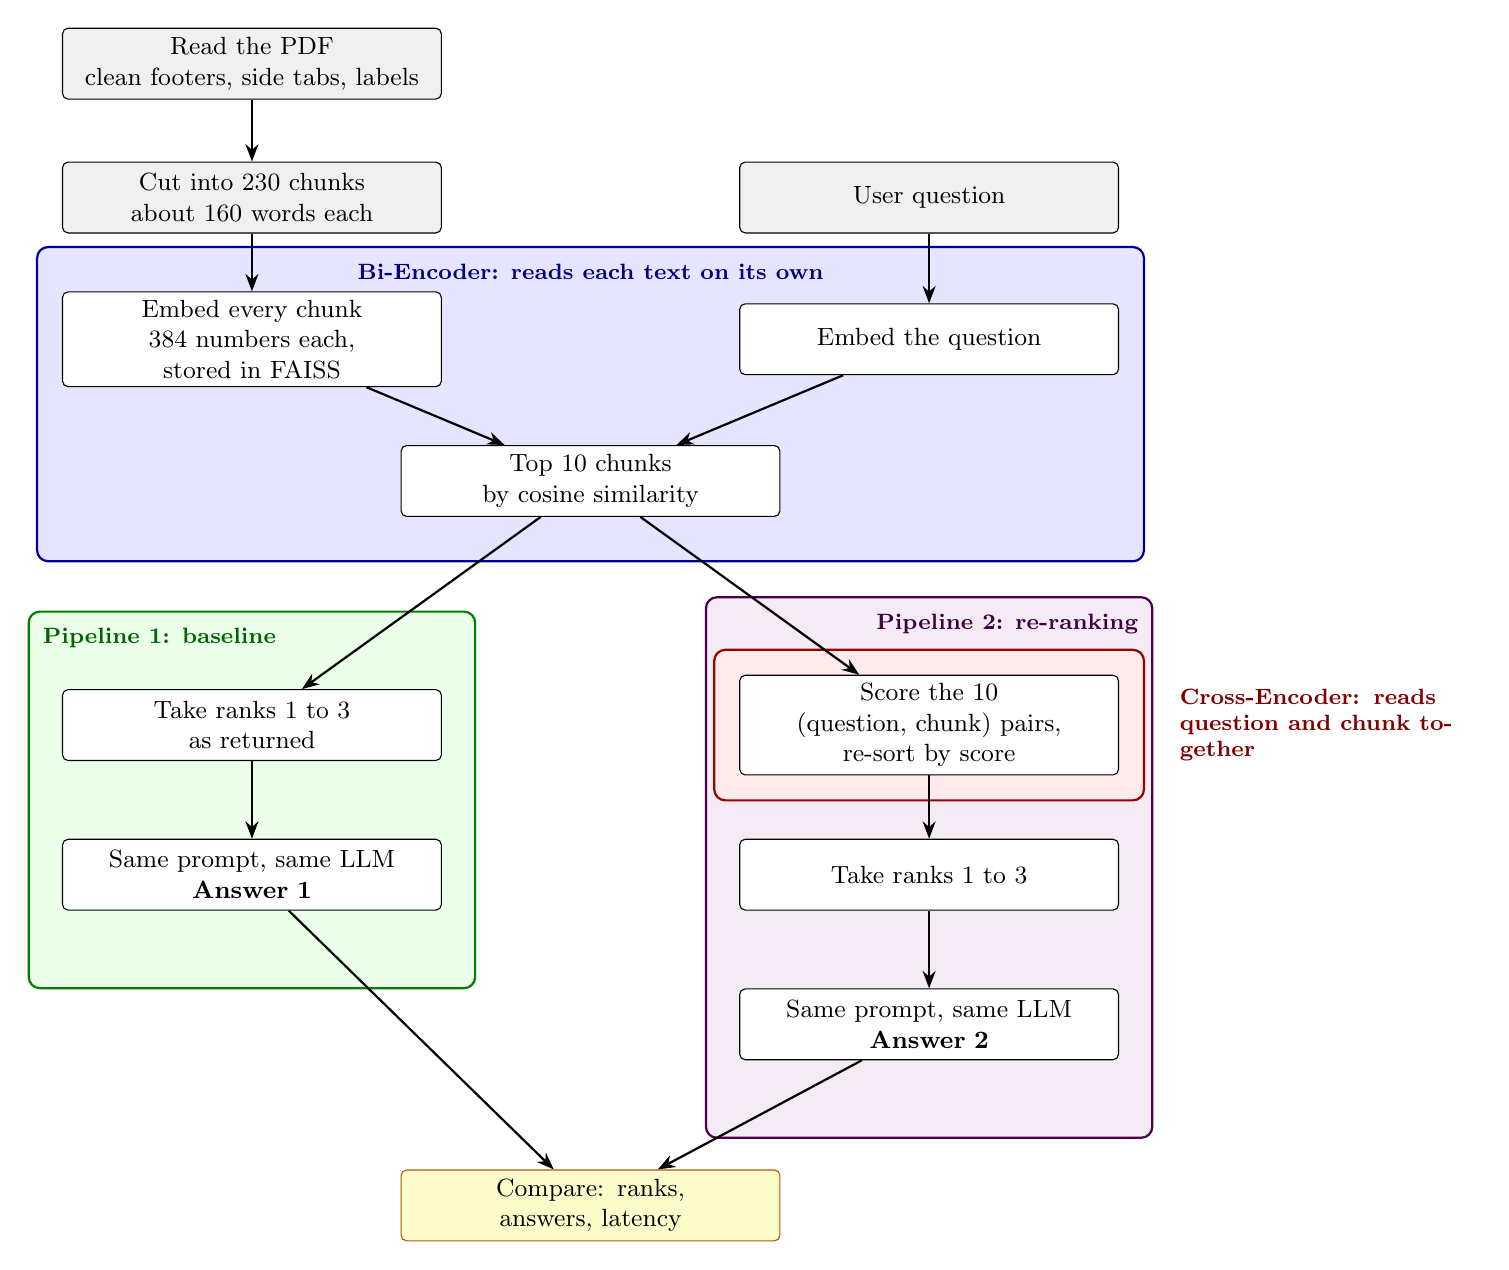
\begin{tikzpicture}[
    font=\small,
    node distance=0.9cm,
    box/.style={draw, rounded corners=2pt, fill=white, align=center, minimum height=0.9cm,
                text width=4.6cm, inner sep=3pt},
    io/.style={box, fill=gray!12},
    result/.style={box, fill=yellow!20, draw=orange!70!black},
    arr/.style={-{Stealth[length=2.2mm]}, thick},
    region/.style={draw, rounded corners=4pt, thick, inner sep=9pt}
  ]
  % --- preparation of the corpus
  \node[io] (pdf)    at (-4.3, 0)    {Read the PDF\\clean footers, side tabs, labels};
  \node[io] (chunks) at (-4.3,-1.7)  {Cut into 230 chunks\\about 160 words each};
  \node[io] (query)  at ( 4.3,-1.7)  {User question};
  % --- Bi-Encoder stage
  \node[box] (emb)   at (-4.3,-3.5)  {Embed every chunk\\384 numbers each, stored in FAISS};
  \node[box] (qemb)  at ( 4.3,-3.5)  {Embed the question};
  \node[box] (top10) at ( 0  ,-5.3)  {Top 10 chunks\\by cosine similarity};
  % --- Pipeline 1 and Pipeline 2
  \node[box] (p1)    at (-4.3,-8.4)  {Take ranks 1 to 3\\as returned};
  \node[box] (score) at ( 4.3,-8.4)  {Score the 10\\(question, chunk) pairs,\\re-sort by score};
  \node[box] (p2)    at ( 4.3,-10.3)  {Take ranks 1 to 3};
  \node[box] (l1)    at (-4.3,-10.3)  {Same prompt, same LLM\\\textbf{Answer 1}};
  \node[box] (l2)    at ( 4.3,-12.2) {Same prompt, same LLM\\\textbf{Answer 2}};
  \node[result] (cmp) at ( 0  ,-14.5) {Compare: ranks, answers, latency};

  % --- coloured regions drawn behind the nodes (outer boxes first, so inner boxes sit on top)
  \begin{scope}[on background layer]
    \node[region, inner xsep=12pt, inner ysep=28pt, fill=green!8, draw=green!50!black, fit=(p1)(l1),
          label={[anchor=north west, green!40!black, font=\footnotesize\bfseries, xshift=2pt, yshift=-3pt]north west:Pipeline 1: baseline}] (pipe1) {};
    \node[region, inner xsep=12pt, inner ysep=28pt, fill=violet!8, draw=violet!60!black, fit=(score)(p2)(l2),
          label={[anchor=north east, violet!50!black, font=\footnotesize\bfseries, xshift=-2pt, yshift=-3pt]north east:Pipeline 2: re-ranking}] (pipe2) {};
    \node[region, inner ysep=16pt, fill=blue!10, draw=blue!60!black, fit=(emb)(qemb)(top10),
          label={[anchor=north, blue!50!black, font=\footnotesize\bfseries, yshift=-3pt]north:Bi-Encoder: reads each text on its own}] (bi) {};
    \node[region, fill=red!8, draw=red!60!black, fit=(score)] (cross) {};
  \end{scope}
  \node[anchor=west, text width=3.7cm, align=left, red!50!black, font=\footnotesize\bfseries]
       at ([xshift=6pt]pipe2.east |- cross.east) {Cross-Encoder: reads question and chunk together};

  % --- arrows
  \draw[arr] (pdf)    -- (chunks);
  \draw[arr] (chunks) -- (emb);
  \draw[arr] (query)  -- (qemb);
  \draw[arr] (emb)    -- (top10);
  \draw[arr] (qemb)   -- (top10);
  \draw[arr] (top10)  -- (p1);
  \draw[arr] (top10)  -- (score);
  \draw[arr] (score)  -- (p2);
  \draw[arr] (p1)     -- (l1);
  \draw[arr] (p2)     -- (l2);
  \draw[arr] (l1)     -- (cmp);
  \draw[arr] (l2)     -- (cmp);
\end{tikzpicture}}
\caption{The two pipelines. Both pipelines share the Bi-Encoder stage; only the selection of the three chunks differs.}
\label{fig:pipelines}
\end{figure}

This assignment builds a question-answering system based on retrieval-augmented generation (RAG): the passages
most relevant to a question are first retrieved from a document, and a language model then answers using only
those passages. The source is a single PDF, the \textit{Laws of the Game 2024/25} published by the International
Football Association Board (IFAB), which has 116 pages. It is a dense rulebook, full of conditions, restrictions
and exceptions. The 20 sections used (Laws 1 to 17, the notes and modifications, the VAR protocol and the
practical guidelines for match officials) contain 26,693 words, in which ``if'' occurs 286 times, ``must'' 227
times, ``unless'' 44 times and ``except'' 29 times.

After the text was cleaned and cut into 230 chunks and each chunk was converted into a vector, two pipelines were
built over the same chunks. Pipeline~1 (baseline) retrieves the ten closest chunks with a Bi-Encoder and passes the
top three to the LLM. Pipeline~2 takes the same ten chunks, re-ranks them with a Cross-Encoder and passes its top
three. The LLM, the prompt and the settings are identical in both pipelines, so any difference in the answers
comes from which three chunks were selected.

The chunk size is limited to about 160 words (the longest chunk has 187) so that chunks stay within the
256-token input limit of the Bi-Encoder; text beyond that limit is ignored by the model. With this tokenizer,
English needs about 1.2 to 1.3 tokens per word (1.21 was measured on this document), so 160 words come to roughly
195 to 210 tokens. One chunk (Law~1, field markings) is still two tokens over the limit once its label is added,
so its last word is not embedded. Both encoders are MiniLM models, each with 6 layers and about 22.7 million
parameters: \texttt{all-MiniLM-L6-v2} (Bi-Encoder) and \texttt{cross-encoder/ms-marco-MiniLM-L-6-v2}
(Cross-Encoder). The vectors are stored in a FAISS flat index, which searches exactly by inner product. The LLM is
\texttt{gemini-3.7-flash}, used through the Gemini API on its free tier. That was sufficient for this project, but
the limit of 20 requests per model per day meant that answers had to be saved and reused. The temperature is 0 so
that the outputs are consistent across runs.

% ============================================================
\section{Architecture Comparison}
% ============================================================

In the Bi-Encoder, each chunk is processed once and on its own, before any question is asked, and the model
produces one vector of 384 numbers for it. The question is encoded separately in the same way. The vectors are
scaled to length 1, so the cosine similarity (the angle between two vectors) can be computed as a simple dot
product, and the chunks are ordered by how close their vectors are to the vector of the question.

In the Cross-Encoder, the question and one chunk are passed together as a single input, so self-attention runs
across the tokens of both texts at once. The output is a single relevance score for each (question, chunk) pair,
and it is used only to order the ten candidates.

Both models have the same MiniLM size, so the difference lies in how they are used and trained. The Bi-Encoder was
trained on about a billion sentence pairs to place related texts close together. The Cross-Encoder was trained on
MS MARCO passage ranking to score relevance directly. Because the Bi-Encoder encodes a chunk without knowing the
question, details such as ``except a goalkeeper'' can be lost in a single vector. The Cross-Encoder can compare the
words of the question with those of the chunk directly, but it must run once for every pair.

% ============================================================
\section{Qualitative and Rank Shift Analysis}
% ============================================================

\subsection{Rank Changes for the Failure Queries}

\begin{table}[H]
\centering
\footnotesize
\renewcommand{\arraystretch}{1.15}
\begin{tabularx}{\textwidth}{@{}l l X c c c@{}}
\toprule
ID & Query type & Question & \shortstack{Rank,\\Pipeline 1} & \shortstack{Rank,\\Pipeline 2} & \shortstack{Moved into\\top 3} \\
\midrule
\rowcolor{green!12}q1 & keyword trap & Can a goal be scored directly from a kick-off? & 5 & 1 & Yes \\
\rowcolor{green!12}q2 & exception & Is a goalkeeper sent off for handling the ball inside their own penalty area to stop a goal? & 9 & 1 & Yes \\
\rowcolor{green!12}q3 & negation & A player is in an offside position but does not touch the ball; is it an offence? & 8 & 1 & Yes \\
\rowcolor{green!12}q4 & vocabulary gap & What if the ball bursts during a match? & 6 & 1 & Yes \\
q5 & control & Can a player wear a ring or a bracelet during a match? & 1 & 1 & No \\
q6 & control & What is the minimum number of players a team needs for the match to continue? & 1 & 1 & No \\
q7 & other & If a player is injured, can the referee give that player a yellow or red card? & 6 & 5 & No \\
\rowcolor{gray!15}q8 & not covered & Can a player bring a water bottle inside the pitch area? & --- & --- & --- \\
\rowcolor{green!12}q9 & vocabulary gap & Can the goalkeeper join the team for the penalty shoot-out at the other team's area? & 10 & 2 & Yes \\
q10 & partly covered & How many red cards can be given to a team in a match and in a tournament? & 2 & 1 & No \\
q11 & negation & Can the coach join for the penalty shoot-out? & 1 & 1 & No \\
\rowcolor{gray!15}q12 & partly covered & If a player is hurt by the ball, is the player who kicked it given a penalty? & $>10$ & $>10$ & No \\
q13 & other & What happens if a player removes their jersey after a goal? & 2 & 2 & No \\
\rowcolor{gray!15}q14 & vocabulary gap & Can a player change their jersey in the middle of a game? & $>10$ & $>10$ & No \\
q15 & other & If a ball went in and then came out, is it a goal? & 1 & 2 & No \\
\bottomrule
\end{tabularx}
\caption{Position of the gold chunk among the ten retrieved chunks. Only ranks 1 to 3 reach the LLM. Green rows: the chunk was outside the top 3 for Pipeline 1 and inside it for Pipeline 2. Grey rows: no rank is available ($>10$ means the chunk was not among the ten candidates; q8 has no gold chunk because the document does not cover the question).}
\label{tab:ranks}
\end{table}

\begin{table}[H]
\centering
\small
\begin{tabular}{@{}l cc cc@{}}
\toprule
 & \multicolumn{2}{c}{All 14 answerable queries} & \multicolumn{2}{c}{12 queries without the controls} \\
\cmidrule(lr){2-3}\cmidrule(lr){4-5}
Metric & Pipeline 1 & Pipeline 2 & Pipeline 1 & Pipeline 2 \\
\midrule
Recall@3 & 0.429 & 0.786 & 0.333 & 0.750 \\
MRR & 0.419 & 0.693 & 0.322 & 0.642 \\
\bottomrule
\end{tabular}
\caption{Recall@3 and mean reciprocal rank (MRR) of the gold chunk. q8 is left out because it has no gold chunk. A gold chunk that is not among the ten candidates counts as a miss.}
\label{tab:metrics}
\end{table}

Pipeline~2 improved the position of the gold chunk for several queries. Among the 14 queries that have a gold
chunk, the gold chunk was in the top three for 6 queries with Pipeline~1 and for 11 with Pipeline~2. It moved from
outside the top three into it for five queries (q1: 5 to 1, q2: 9 to 1, q3: 8 to 1, q4: 6 to 1, q9: 10 to 2),
and the two controls (q5, q6) stayed at rank 1. In q15 the gold chunk moved down from rank 1 to rank 2, which is
still inside the top three.

Some queries could not be improved. For q12 and q14 the gold chunk was not among the ten candidates, so
re-ranking could not help, because it can only reorder those ten. In q7 the gold chunk moved only from rank 6 to
rank 5, which is still outside the top three. Query q8 has no gold chunk, since the Laws do not mention water
bottles on the field. Rewording the questions helped in some cases: 11 of the 16 rewrites moved the gold chunk to a
different rank (Table~\ref{tab:rewrites}).

\subsection{Answer 1 versus Answer 2}

\begin{table}[H]
\centering
\footnotesize
\renewcommand{\arraystretch}{1.15}
\begin{tabularx}{\textwidth}{@{}l X c c@{}}
\toprule
ID & Question & Answer 1 (Pipeline 1) & Answer 2 (Pipeline 2) \\
\midrule
q1 & Can a goal be scored directly from a kick-off? & Refused & Answered \\
q2 & Is a goalkeeper sent off for handling the ball inside their own penalty area to stop a goal? & Refused & Answered \\
q3 & A player is in an offside position but does not touch the ball; is it an offence? & Refused & Answered \\
q4 & What if the ball bursts during a match? & Refused & Answered \\
q5 & Can a player wear a ring or a bracelet during a match? & Answered & Answered \\
q6 & What is the minimum number of players a team needs for the match to continue? & Answered & Answered \\
q7 & If a player is injured, can the referee give that player a yellow or red card? & Refused & Refused \\
q8 & Can a player bring a water bottle inside the pitch area? & Refused & Refused \\
q9 & Can the goalkeeper join the team for the penalty shoot-out at the other team's area? & Refused & Refused \\
q10 & How many red cards can be given to a team in a match and in a tournament? & Refused & Refused \\
q11 & Can the coach join for the penalty shoot-out? & Refused & Refused \\
q12 & If a player is hurt by the ball, is the player who kicked it given a penalty? & Refused & Refused \\
q13 & What happens if a player removes their jersey after a goal? & Answered & Answered \\
q14 & Can a player change their jersey in the middle of a game? & Refused & Refused \\
q15 & If a ball went in and then came out, is it a goal? & Refused & Refused \\
\bottomrule
\end{tabularx}
\caption{Whether the LLM gave an answer or replied ``The context does not contain the answer.'' This records only the reply type, not whether an answer is correct. The full answers are in \texttt{results/answers.json}.}
\label{tab:answers}
\end{table}

With Pipeline~1 the LLM answered only 3 of the 15 queries (q5, q6 and q13) and replied that the context did not
contain the answer for the other 12. With Pipeline~2 it answered 7 of the 15 (q1 to q6 and q13), almost half. For
the failure queries q1 to q4, the gold chunk was outside the top three of Pipeline~1, so its refusal is an
omission caused by retrieval and not an invented answer. No hallucination was found: the answers that were given
agree with the text of the retrieved chunks.

Not every refusal comes from retrieval. For q10, q11 and q15 the gold chunk was already in the top three of both
pipelines, yet the LLM still refused. The refusal for q8 is correct, because the Laws are silent on the question.

The answer to the rewritten question q9r2 is incomplete. It says that a goalkeeper can take a kick in a penalty
shoot-out and that a replaced goalkeeper may not, but it does not say that an eligible player may change places
with the goalkeeper (Law~10), although that chunk was in its context. It also omits the conditions in Law~3: the
referee must be informed and the change must be made during a stoppage. Such a change leaves the goal without its
goalkeeper. The other answers were satisfactory.

\begin{table}[H]
\centering
\footnotesize
\renewcommand{\arraystretch}{1.15}
\begin{tabularx}{\textwidth}{@{}l X c c c c@{}}
\toprule
ID & Rewritten question & \shortstack{Original rank\\P1 / P2} & \shortstack{New rank\\P1 / P2} & \shortstack{Answer 1} & \shortstack{Answer 2} \\
\midrule
q7r1 & Can the referee caution or send off a player who is injured? & 6 / 5 & 6 / 1 & Refused & Answered \\
q7r2 & Does an injured player get a card from the referee? & 6 / 5 & 2 / 1 & --- & --- \\
q7r3 & Can a player who is hurt and leaving the pitch for treatment be shown a yellow or red card? & 6 / 5 & 4 / 3 & --- & --- \\
q9r1 & Can an outfield player take the goalkeeper's place during a penalty shoot-out? & 10 / 2 & $>10$ / $>10$ & --- & --- \\
q9r2 & Can the goalkeeper take a penalty kick in a shoot-out? & 10 / 2 & 6 / 2 & Answered & Answered \\
q10r1 & Is there a limit on how many players of one team can be sent off? & 2 / 1 & 1 / 1 & Refused & Refused \\
q10r2 & What happens if too many players of a team are sent off? & 2 / 1 & 1 / 3 & --- & --- \\
q11r1 & Are team officials allowed on the field during the penalty shoot-out? & 1 / 1 & 2 / 1 & Answered & Answered \\
q11r2 & Who is allowed on the pitch during a penalty shoot-out? & 1 / 1 & 2 / 1 & --- & --- \\
q14r2 & What must a player do to change their kit during a match? & $>10$ / $>10$ & 9 / 1 & Refused & Answered \\
q15r2 & If the ball crosses the goal line and then returns to the field, is a goal given? & 1 / 2 & 1 / 1 & Refused & Refused \\
\bottomrule
\end{tabularx}
\caption{Effect of rewording the question. The gold chunk is unchanged; only the wording differs. Of 16 rewrites tried, the 11 shown here moved the gold chunk to a different rank in at least one pipeline (the other 5 left it where it was). The rewrites were written after the original results were seen, so this shows sensitivity to wording and is not an independent test. To stay within the free API limit, the LLM was asked for one rewrite per original query only (``---'' means not asked). P1 and P2 are Pipelines 1 and 2. $>10$ means the gold chunk was not among the ten candidates.}
\label{tab:rewrites}
\end{table}

Rewording changed the outcome for four of the six queries for which the LLM was asked again. For q7r1 and q14r2 only
Pipeline~2 produced an answer, and for q9r2 and q11r1 both pipelines did, where the original wording had been
refused. The rewrites q10r1 and q15r2 were still refused. The rewrites were written after the original results
were seen, so this shows how sensitive the system is to wording and is not an independent test.

% ============================================================
\section{Latency Profiling}
% ============================================================

\begin{table}[H]
\centering
\small
\renewcommand{\arraystretch}{1.15}
\begin{tabular}{@{}l r r@{}}
\toprule
Step & Pipeline 1 (ms) & Pipeline 2 (ms) \\
\midrule
Bi-Encoder retrieval (embed the question, search 230 chunks) & 8.6 & 8.6 \\
Cross-Encoder re-ranking of the 10 candidates & --- & 99.3 \\
\midrule
Retrieval total (local CPU) & 8.6 & 107.8 \\
\midrule
LLM call, Gemini API (median, includes network), s & 4.00 & 5.13 \\
\bottomrule
\end{tabular}
\caption{Median runtime per query on the CPU, after a warm-up pass, over 15 queries with 5 repeats each (75 timings). The LLM time is a network call, was measured when each answer was first generated, and is not comparable with the local steps.}
\label{tab:latency}
\end{table}

Pipeline~1 takes 8.6~ms for retrieval (embedding the question and searching the 230 chunks). Pipeline~2 adds
99.3~ms for the Cross-Encoder, which gives 107.8~ms in total. As expected, the retrieval of Pipeline~1 takes less
than a tenth of the time of Pipeline~2 (about 8\%), because the Cross-Encoder runs a full pass for each of the ten
pairs, at about 10~ms per pair. The LLM call takes seconds in both pipelines (median 4.00~s and 5.13~s, including
network time) and dominates the total, but it is not comparable with the local steps.

% ============================================================
\section{Scaling Question}
% ============================================================

The Cross-Encoder needs one forward pass for every (question, chunk) pair, and nothing can be computed in advance,
because the score depends on the question. The Bi-Encoder encodes every chunk once, before any question is asked,
so a query costs only one embedding of the question and one similarity search. At the measured 10~ms per pair,
scoring all 230 chunks would take about 2.3~s per question instead of about 0.1~s for ten pairs. The cost grows in
proportion to the size of the collection: as an estimate from the same figure, one million chunks would need about
2.8 hours per question on this CPU. The Bi-Encoder is therefore used to shortlist quickly, and the slower but more
careful Cross-Encoder is applied only to that shortlist.

\end{document}
